\documentclass[11pt,a4paper]{article}
\usepackage[spanish,es-nodecimaldot]{babel}	% Utilizar español
\usepackage[utf8]{inputenc}					% Caracteres UTF-8
\usepackage{graphicx}						% Imagenes
\usepackage[hidelinks]{hyperref}			% Poner enlaces sin marcarlos en rojo
\usepackage{fancyhdr}						% Modificar encabezados y pies de pagina
\usepackage{float}							% Insertar figuras
\usepackage[textwidth=390pt]{geometry}		% Anchura de la pagina
\usepackage[nottoc]{tocbibind}				% Referencias (no incluir num pagina indice en Indice)
\usepackage{enumitem}						% Permitir enumerate con distintos simbolos
\usepackage[T1]{fontenc}					% Usar textsc en sections
\usepackage{amsmath}						% Símbolos matemáticos
\usepackage{pdflscape}
\usepackage{typearea} % Paginas horizontales

% Comando para poner el nombre de la asignatura
\newcommand{\asignatura}{Sistemas Gráficos}
\newcommand{\autor}{Vladislav Nikolov Vasilev}
\newcommand{\titulo}{Pac-Man 3D}
\newcommand{\subtitulo}{Diseño de la aplicación}
\newcommand{\rama}{Ingeniería del Software}

% Configuracion de encabezados y pies de pagina
\pagestyle{fancy}
\lhead{\autor{}}
\rhead{\asignatura{}}
\lfoot{Grado en Ingeniería Informática}
\cfoot{}
\rfoot{\thepage}
\renewcommand{\headrulewidth}{0.4pt}		% Linea cabeza de pagina
\renewcommand{\footrulewidth}{0.4pt}		% Linea pie de pagina

% new pagestyle
\fancypagestyle{lscape}{
  \headwidth\textwidth
}

\begin{document}
\pagenumbering{gobble}

% Pagina de titulo
\begin{titlepage}

\begin{minipage}{\textwidth}

\centering

%
\includegraphics[scale=0.5]{img/ugr.png}\\

\includegraphics[scale=0.3]{img/logo_ugr.jpg}\\[1cm]

\textsc{\Large \asignatura{}\\[0.2cm]}
\textsc{GRADO EN INGENIERÍA INFORMÁTICA}\\[1cm]

\noindent\rule[-1ex]{\textwidth}{1pt}\\[1.5ex]
\textsc{{\Huge \titulo\\[0.5ex]}}
\textsc{{\Large \subtitulo\\}}
\noindent\rule[-1ex]{\textwidth}{2pt}\\[3.5ex]

\end{minipage}

%\vspace{0.5cm}
\vspace{0.7cm}

\begin{minipage}{\textwidth}

\centering

\textbf{Autor}\\ {\autor{}}\\[2.5ex]
\textbf{Rama}\\ {\rama}\\[2.5ex]
\vspace{0.3cm}


\includegraphics[scale=0.3]{img/etsiit.jpeg}

\vspace{0.7cm}
\textsc{Escuela Técnica Superior de Ingenierías Informática y de Telecomunicación}\\
\vspace{1cm}
\textsc{Curso 2019-2020}
\end{minipage}
\end{titlepage}

\pagenumbering{arabic}
\tableofcontents
\thispagestyle{empty}				% No usar estilo en la pagina de indice

% start new page before setting page layout,
% otherwise previous page is also affected
\KOMAoption{paper}{landscape}%
\typearea{12}% sets new DIV

% Establecer pagina horizontal
\recalctypearea
% needed to show page in landscape in viewer
\pdfpageheight=\paperheight
\pdfpagewidth=\paperwidth
% Poner estilo
\pagestyle{lscape}


\setlength{\parskip}{1em}

\section{Diagrama de clases}

\begin{figure}[H]
  \centering
  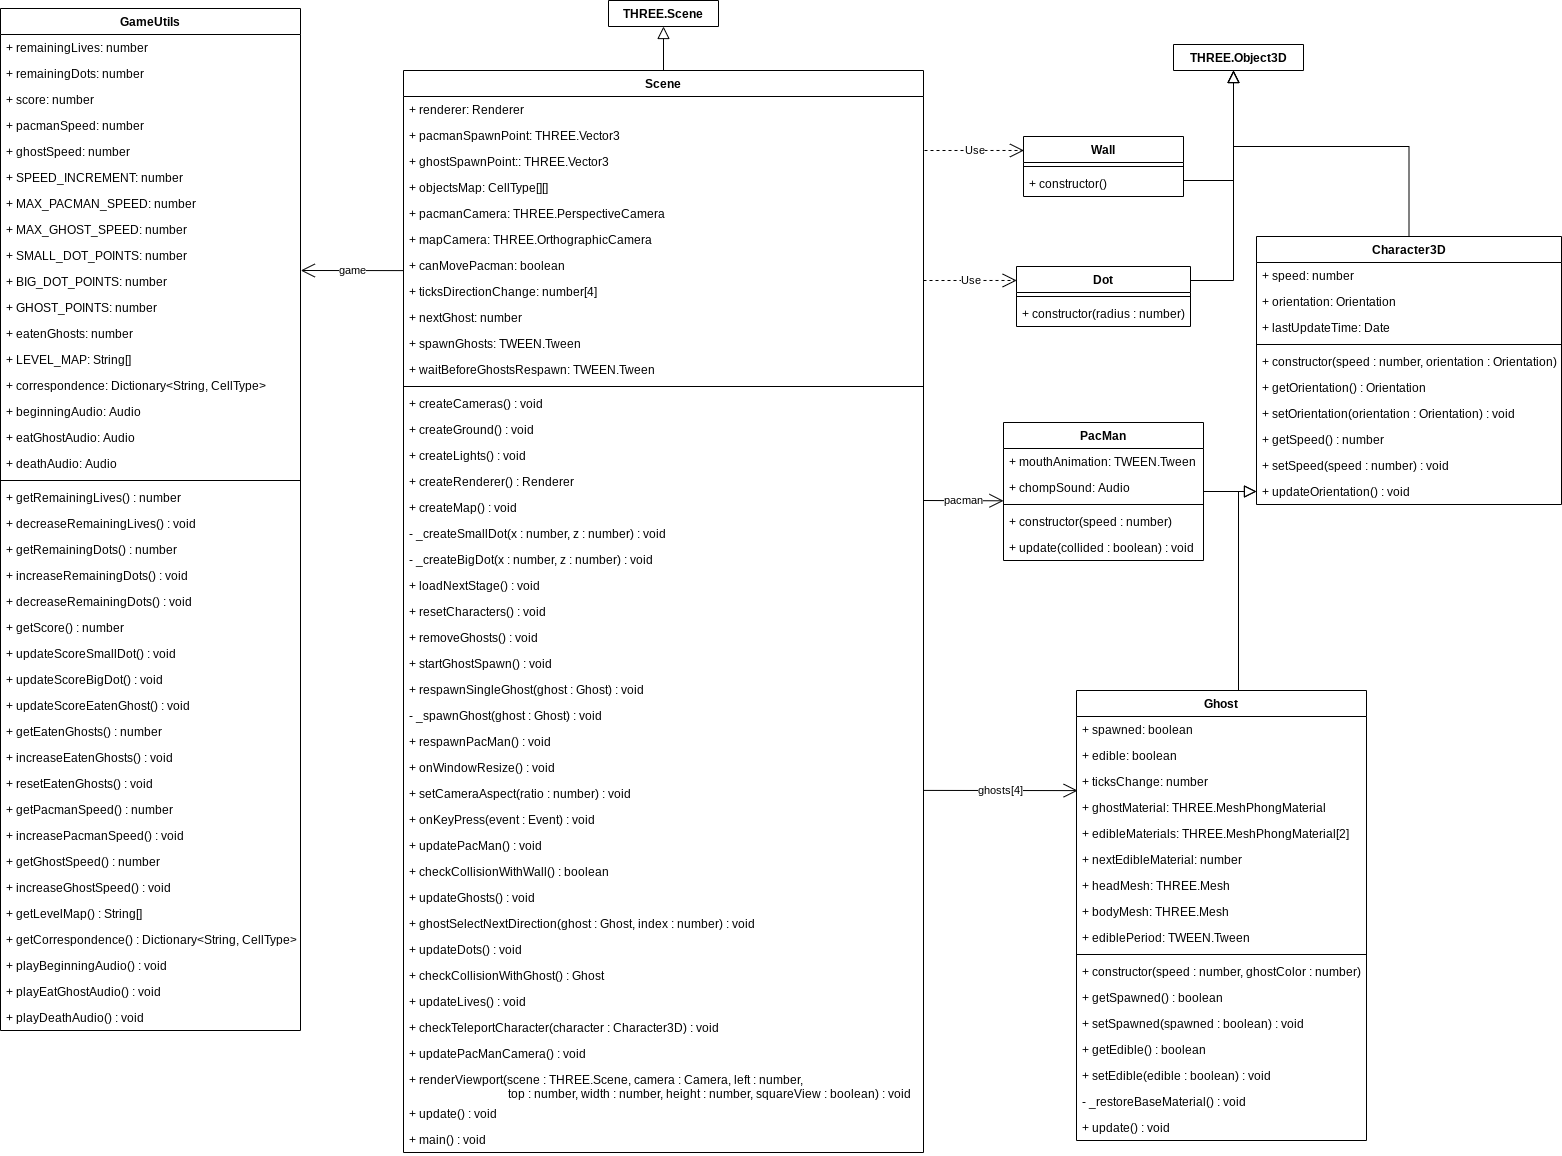
\includegraphics[scale=0.365]{img/diagrama-clases}
\end{figure}

\KOMAoptions{paper=portrait}
\recalctypearea
\pdfpageheight=\paperheight
\pdfpagewidth=\paperwidth
\headwidth\textwidth

Partiendo del diagrama de clases anterior, vamos a describir algunas de las clases para que
se entienda qué representa cada una de ellas.

\newpage

\begin{thebibliography}{5}

\bibitem{nombre-referencia}
Texto referencia
\\\url{https://url.referencia.com}

\end{thebibliography}

\end{document}

